
    \begin{abstract_online}{Oil Detachment from Rock Surface using Nanoparticle, Surfactant and Low Salinity Brine: A Molecular Dynamic Study}{%
        \underline{R. Kashyap}$^{1}$, R. Kumar$^{2}$, N. M. A. Krishnan$^{2}$, A. Kashyap$^{1}$}{%
        }{%
        $^1$ School of Basic Science, IIT Mandi, Mandi, H.P. India \newline{}$^2$  Department of Civil Engineering, IIT Delhi, New Delhi, India }
    Chemical enhanced oil recovery (EOR) is a promising method to meet the continuous increase in oil demand and keep sustainable oil supply [1]. Nanomaterials, surfactants and ions have received major attention due to their potential application in EOR[2]. The main function of these materials is to help in wettability alteration, reduces interfacial tension, increasing viscosity of water, self-cleansing agent, etc. which finally results in destabilizing the oil layer at rock surface causing easy oil recovery[3]. \par  We investigated the oil detachment mechanism from the sandstone surface using nanoparticle, brine water of low concentration and surfactant using molecular dynamic simulation as shown in Fig.1. Through analysis of all ionic, atomic and molecular force field and surface interaction between rock -fluid  were done at reservoir operating conditions. The result showed that both surfactant and nanoparticle are adsorbed at oil and brine interface which reduces the interfacial tension and increases the total surface pressure resulting in oil detachment. Synergistic effect of ionic species, surfactant and nanoparticles on wettability alteration of rock surface from oil-wet to water-wet condition were also investigated. Our molecular simulation study provided information on the oil detachment from the rock surface. This is useful for petroleum industries to understand the underlying mechanism of complex injecting fluid for optimal oil recovery which will play a major role in future oil supply. \begin{center}  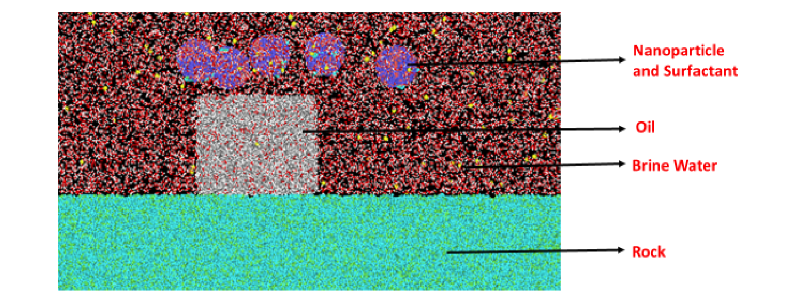
\includegraphics[width=\linewidth]{abstracts/txt/figures/rajneesh.png}  \caption{Simulation model schematic diagram}  \end{center}  
    
        \textbf{References} \newline{}[1] Bartels W-B, et al., Fuel, 2019, 236, 338–53.\newline{}[2] D. Wu, et al., Langmuir, 34, 2017, 1225–1233.\newline{}[3] Tian H, Wang M., Surf Sci Rep, 2017, 72, 369–91.
    \end{abstract_online}
    